\documentclass{reporti}

\titulo{Trabajo Práctico. Diseño individual de una PCI}
\subtitulo{Diseño PCB}
\autor{J. L. Benavides - \href{mailto:jorge2@uma.es}{jorge2@uma.es}}
\contact{\href{mailto:jorge2@uma.es}{Feedback sobre la documentación}}
\logo{rhyloo_solutions_horizontal.pdf}

\type{Reporte de resultados}
\code{ALLIO\_PCB\_V0.0}

\resumen{The TAS5518-5261K2EVM PurePath Digital™ customer evaluation module demonstrates the integrated circuits TAS5518PAG and TAS5261DKD from Texas Instruments (TI). This application report covers the TAS5518-5261EVM PurePath Digital™ evaluation module specifications, audio performance and power efficiency measurements graphs, and design documentation that includes schematics, parts list, layout, and mechanical design.}

\notes{PurePath Digital, Equibit are trademarks of Texas Instruments.\\ Excel is a trademark of Microsoft Corporation.}

\begin{document}
\cover[width=1.35\textwidth]
\tableofcontents
\listoffigures
\listoftables

\section{Dimensiones y posicionamiento}
\subsection{test}
\begin{figure}[h]
  \centering
  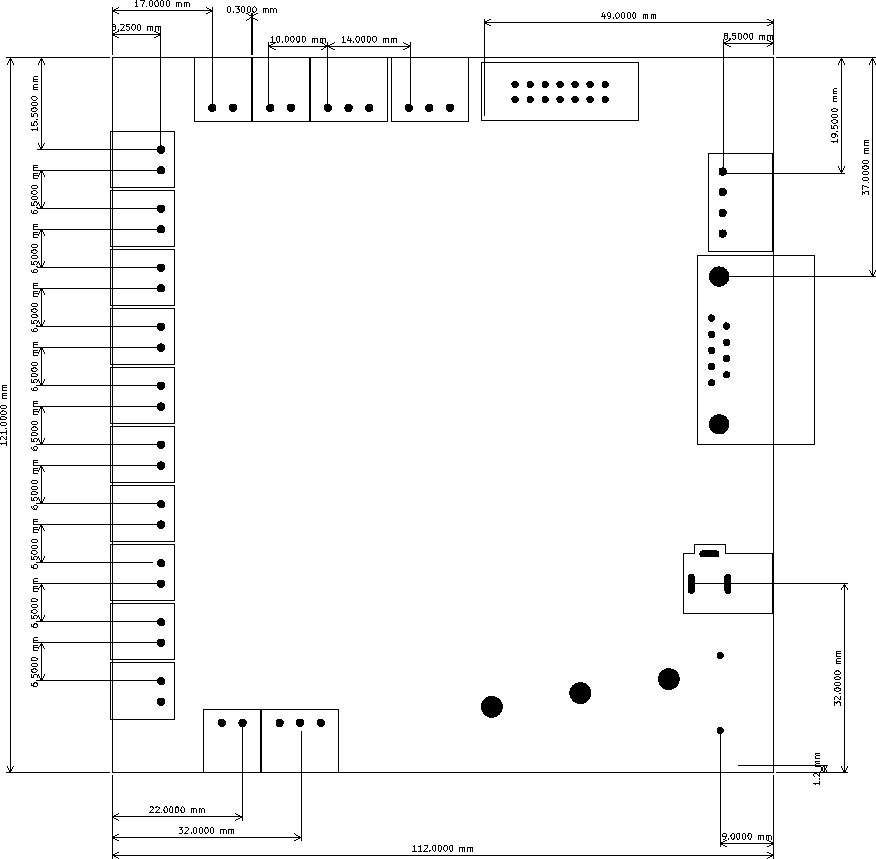
\includegraphics[scale=1]{PCB_dimensiones.pdf}
  \caption{Posición de los componentes.}
\end{figure}

\section{Especificaciones de fabricación}
\begin{table}[H]
  \centering
  \begin{tabularx}{\textwidth}{lX}
    \toprule
    \textbf{Sección} & \textbf{Detalle} \\
    \midrule

    \multirow{2}{*}{\textbf{Identificación}} 
    & Código de referencia: ALLIO\_PCB\_V0.0 \\
    & Revisión: V0.0 \\
    \cmidrule(lr){1-2}

    \multirow{3}{*}{\textbf{Detalles generales}} 
    & Tiempo de fabricación deseado: 1 mes \\
    & Dimensiones de la PCB: 112 mm × 121 mm \\
    & Número de placas: 5 unidades (sin panelización) \\
    \cmidrule(lr){1-2}

    \multirow{12}{*}{\textbf{Especificaciones técnicas}} 
    & Espesor total de la PCB: 1.6 mm \\
    & Espesor de cobre externo: 0.035 mm (1 oz) \\
    & Espesor de cobre interno: No aplica (2 capas) \\
    & Número de capas: 2 \\
    & Material base: FR4 \\
    & FR4-TG: TG 130-140 \\
    & Acabado superficial: Níquel por inmersión \\
    & Color de la máscara de soldadura: Negro \\
    & \textbf{Serigrafía:} \\
    & \quad • Color silkscreen: Blanco \\
    & \quad • Capas con serigrafía: 2 (ambos lados) \\
    & \quad • Alto mínimo del texto: 0.8 mm \\
    \cmidrule(lr){1-2}

    \textbf{Parámetros de fabricación} & \\
    \multicolumn{2}{l}{\textit{Cobre}} \\
    & \quad • Margen mínimo: 0 mm \\
    & \quad • Ancho mínimo de pista: 0.2 mm \\
    & \quad • Ancho mínimo de conexión: 0 mm \\
    & \quad • Ancho mínimo de anular: 0.05 mm \\
    & \quad • Mínimo diámetro de vía: 0.4 mm \\
    & \quad • Margen de cobre a agujero: 0.25 mm \\
    & \quad • Margen de cobre a borde: 0 mm \\
    \multicolumn{2}{l}{\textit{Orificios}} \\
    & \quad • Orificio pasante mínimo: 0.3 mm \\
    & \quad • Margen de orificio a orificio: 0.25 mm \\
    \multicolumn{2}{l}{\textit{uVias}} \\
    & \quad • Diámetro mínimo de uVia: 0.2 mm \\
    & \quad • Orificio mínimo de uVia: 0.1 mm \\
    & \quad • Via process: Cubiertas (tented) \\
    \multicolumn{2}{l}{\textit{Serigrafía}} \\
    & \quad • Margen mínimo de elemento: 0 mm \\
    & \quad • Alto mínimo del texto: 0.8 mm \\
    \cmidrule(lr){1-2}

    \textbf{Otros requisitos} 
    & Test electrónico: No requerido. \\
    \bottomrule
  \end{tabularx}
\end{table}
\end{document}

LaTeX finished at Sat May 31 22:21:58
